\hspace{1.5cm}
Para ENVI \cite{envi}, realizar a analise temporal de duas imagens é necessário construir a correção geométrica. Isto processo tem fundamental devido aos acidentes geográfico não estarem sobreposto nas imagens. Este metodo basea-se em marcar os pontos de controles nos acidentes, nas duas imagens (imagem-to-imagem).\\

\begin{itemize}
\item Map
\begin{itemize}
\item \textbf{Registration} $\rightarrow$ \textbf{Select GCPs:Image to Image}
\end{itemize}
\begin{figure}[!htpb]
        \centering
        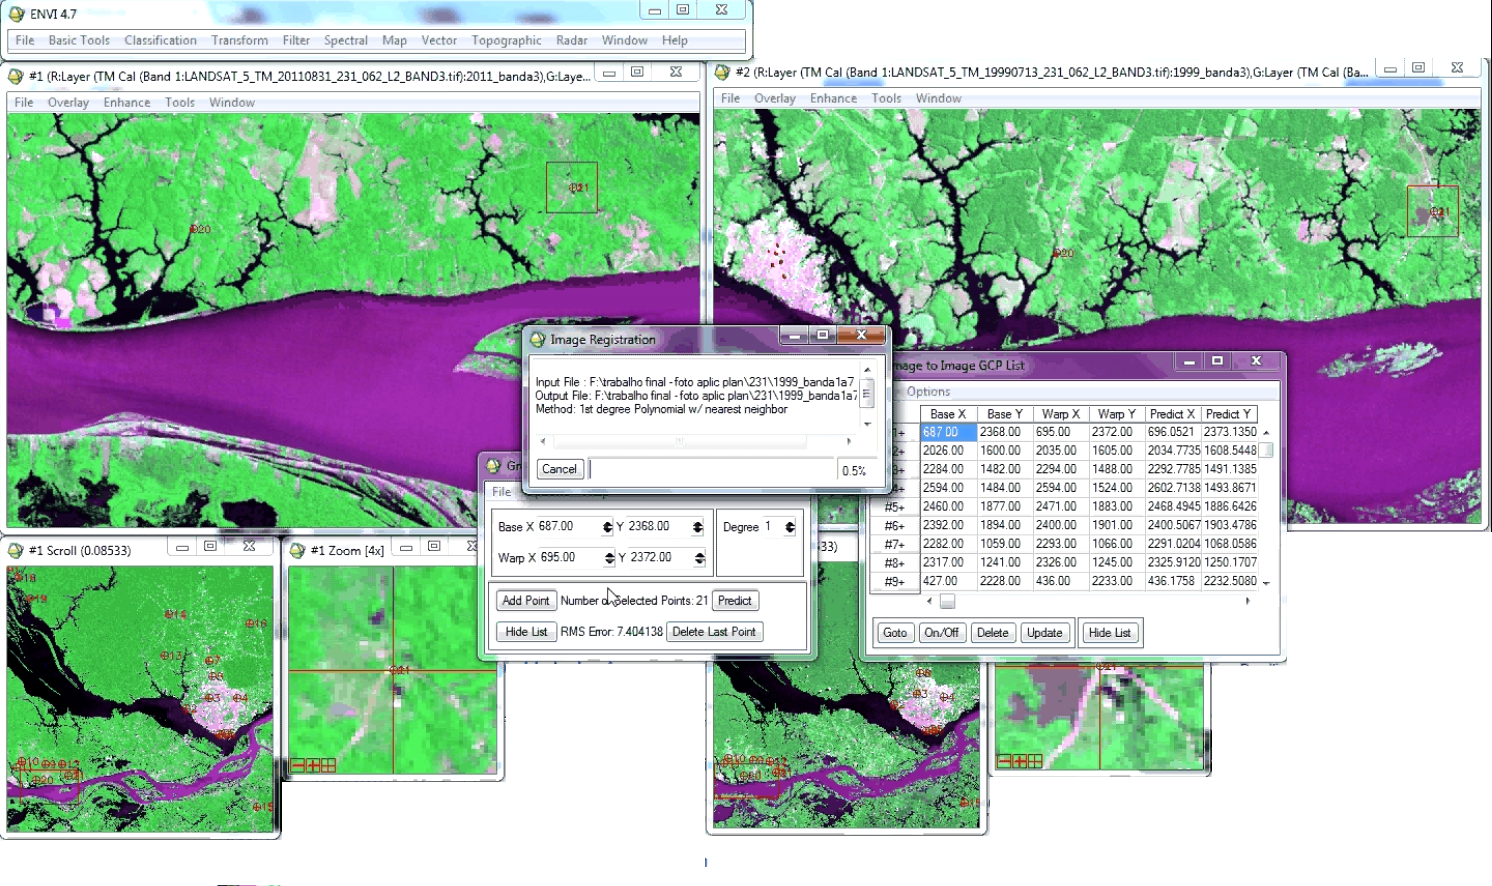
\includegraphics[scale =0.2]{imagens/correcao04a.png}
        \caption{Processo de Correção Geométrica.}
        \label{correcao04}
\end{figure}
\end{itemize}
\hspace{1.5cm}
No nosso processo foram selecionado 20 (vinte) pontos de controles, nas dois compostos de banda. Os pontos são melhores definidos na janela de zoom. Após a coleta de pontos nos acidentes é dado o nome do arquivo "pts" e chamado no \textbf{Map} $\rightarrow$ \textbf{Registration} $\rightarrow$ \textbf{Warp from GCPs:image to Image}, para gerar a correção entre a imagem (base e warp). A figura \ref{correcao04} mostra o processo realizado.

